\documentclass{beamer}
\usepackage[utf8]{inputenc}
\usepackage{graphicx}
\usepackage{booktabs}
\usepackage{hyperref}
\usepackage{amsmath}
\usepackage{tikz}
\usepackage{caption}
\usepackage{float}

\title[P15: IMDb Sentiment Classification]{P15: Sentiment Classification of IMDb Movie Reviews}
\subtitle{CS485 – Project Presentation}
\author{Zervos Spiridon Chrisovalantis (csd4878) \\ Drakakis Rafail (csd5310)}
\date{}
\institute{University of Crete}

\begin{document}

\frame{\titlepage}

\begin{frame}{Project Objectives}
\begin{itemize}
  \item Build a sentiment classification pipeline for IMDb reviews
  \item Apply classical and deep learning models
  \item Evaluate performance: accuracy, speed, and confusion matrices
  \item Analyze model behavior and limitations
\end{itemize}
\end{frame}

\begin{frame}{Dataset Overview}
\begin{itemize}
  \item \textbf{Name:} IMDb Large Movie Review Dataset
  \item \textbf{Size:} 25k train / 25k test reviews
  \item \textbf{Labels:} Binary – Positive (1), Negative (0)
  \item \textbf{Source:} \url{https://ai.stanford.edu/~amaas/data/sentiment/}
\end{itemize}
\end{frame}

\begin{frame}{Text Preprocessing}
\begin{itemize}
  \item Lowercasing, tokenization using NLTK
  \item Removing punctuation, numbers, stopwords
  \item For deep learning:
  \begin{itemize}
    \item Vocabulary built (min frequency = 2, max size = 20,000)
    \item Sequences padded/truncated to 200 tokens
  \end{itemize}
\end{itemize}
\end{frame}

\begin{frame}{Feature Engineering}
\begin{itemize}
  \item \textbf{Classical ML:} TF–IDF vectorization (unigrams, top 5,000 features)
  \item \textbf{Deep Learning:} Trainable embeddings (dimension = 100)
\end{itemize}
\end{frame}

\begin{frame}{Classical Model Configurations}
\begin{itemize}
  \item \textbf{Logistic Regression:} L2 regularization, $C = 1.0$
  \item \textbf{Naïve Bayes:} Multinomial, $\alpha = 1.0$
  \item \textbf{Linear SVM:} $C = 1.0$
\end{itemize}
\end{frame}

\begin{frame}{Deep Learning Architectures}
\textbf{LSTM:}
\begin{itemize}
  \item Single layer, 128 hidden units
  \item Uses final hidden state
\end{itemize}

\vspace{1em}
\textbf{CNN:}
\begin{itemize}
  \item Filters: sizes [3, 4, 5], 100 each
  \item Max pooling and FC layer
\end{itemize}
\end{frame}

\begin{frame}{Training Setup}
\begin{itemize}
  \item Optimizer: Adam, learning rate = $1e^{-3}$
  \item Epochs: 5, Batch size: 64
  \item Implemented in PyTorch
  \item Inference script: \texttt{predict.py} (Can be used to predict new reviews)
\end{itemize}
\end{frame}

\begin{frame}{Classical Model Results}
\begin{table}[H]
\centering
\begin{tabular}{lcc}
\toprule
\textbf{Model} & \textbf{Accuracy} & \textbf{Time (ms/sample)} \\
\midrule
Logistic Regression & 0.880 & 0.47 \\
Naïve Bayes & 0.840 & 0.13 \\
Linear SVM & 0.863 & 0.65 \\
\bottomrule
\end{tabular}
\caption*{TF–IDF features, evaluated on 25k test samples}
\end{table}
\end{frame}

\begin{frame}{Logistic Regression Report}
\begin{itemize}
  \item Precision, Recall, F1-score: 0.88 for both classes
  \item Balanced performance across sentiment labels
  \item Fast inference: 0.47 ms/sample
\end{itemize}
\begin{figure}[H]
\centering
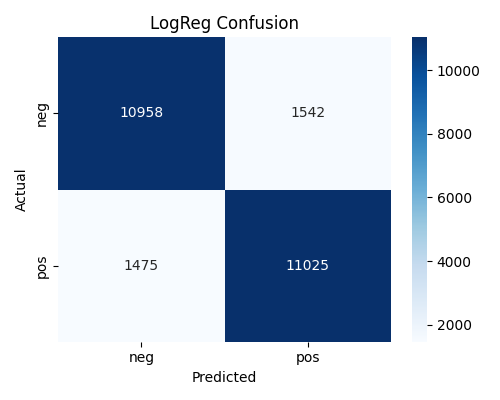
\includegraphics[width=0.5\textwidth]{figures/LogReg_confusion.png}
\caption*{Confusion Matrix: Logistic Regression}
\end{figure}
\end{frame}

\begin{frame}{Deep Learning Results}
\begin{table}[H]
\centering
\begin{tabular}{lcc}
\toprule
\textbf{Model} & \textbf{Accuracy} & \textbf{Notes} \\
\midrule
LSTM & 0.511 & Underfitting, unstable learning \\
CNN & 0.856 & Competitive, robust features \\
\bottomrule
\end{tabular}
\end{table}
\begin{figure}[H]
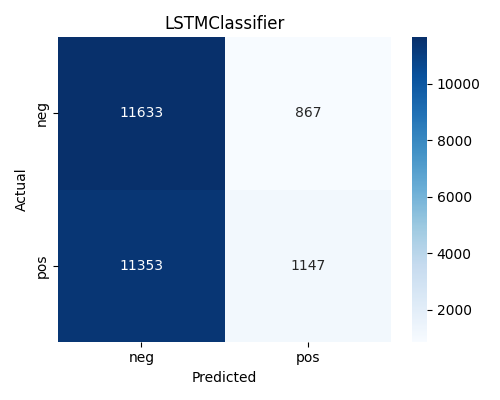
\includegraphics[width=0.45\textwidth]{figures/LSTMClassifier_confusion.png}
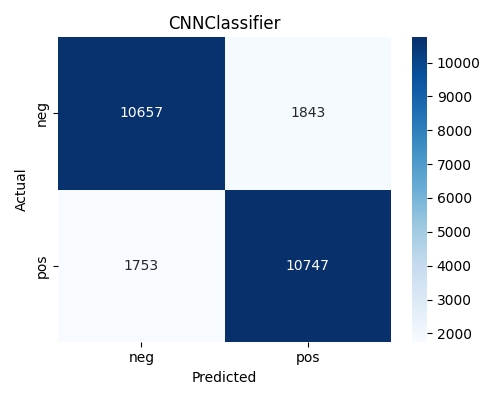
\includegraphics[width=0.45\textwidth]{figures/CNNClassifier_confusion.png}
\caption*{Confusion Matrices: LSTM (left), CNN (right)}
\end{figure}
\end{frame}

\begin{frame}{Model Comparison}
\begin{itemize}
  \item \textbf{Best Accuracy:} Logistic Regression (0.88)
  \item \textbf{Best DL Model:} CNN (0.856)
  \item \textbf{Fastest Inference:} Naïve Bayes (0.13 ms/sample)
  \item \textbf{Underperformer:} LSTM (0.511), due to lack of tuning and pretraining
\end{itemize}
\end{frame}

\begin{frame}{Error Analysis}
\begin{itemize}
  \item \textbf{LSTM:} Poor generalization without pretrained embeddings
  \item \textbf{CNN:} Stronger with local patterns (n-grams)
  \item \textbf{All Models:}
  \begin{itemize}
    \item Misclassify short or sarcastic reviews
    \item Struggle with implicit sentiment
  \end{itemize}
\end{itemize}
\end{frame}

\begin{frame}{Conclusion}
\begin{itemize}
  \item Classical methods remain strong
  \item CNNs show promise with competitive accuracy
  \item LSTM requires optimization: embeddings, attention, deeper networks
\end{itemize}
\end{frame}

\begin{frame}{Q \& A}
\centering
\Huge Questions?
\end{frame}

\end{document}